\documentclass[tikz,border=8pt]{standalone}
\begin{document}
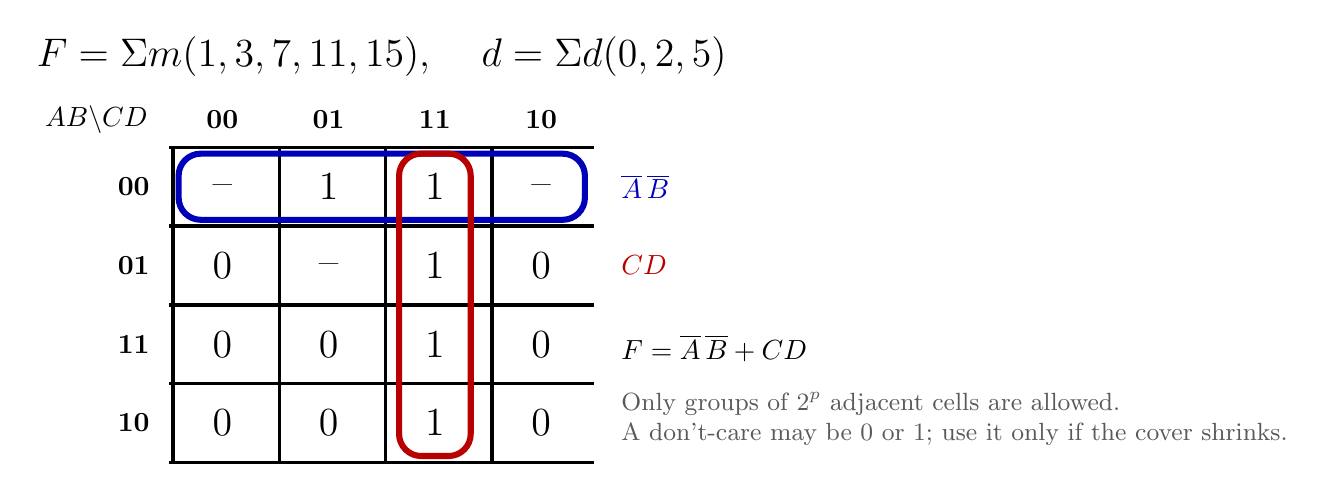
\begin{tikzpicture}[font=\sffamily]
\node[font=\bfseries\Large] at (4.0,6.15)
  {$F=\Sigma m(1,3,7,11,15),\quad d=\Sigma d(0,2,5)$};

% Four-variable map. Rows AB and columns CD use Gray order 00,01,11,10.
\draw[very thick] (1.3,1.0) grid[xstep=1.35,ystep=1.0] (6.7,5.0);
\node[anchor=east,font=\bfseries] at (1.15,5.35) {$AB\backslash CD$};

\foreach \x/\lab in {1.975/00,3.325/01,4.675/11,6.025/10}
  \node[font=\bfseries] at (\x,5.35) {\lab};
\foreach \y/\lab in {4.5/00,3.5/01,2.5/11,1.5/10}
  \node[font=\bfseries] at (.85,\y) {\lab};

% Cell contents by minterm index: dash is a don't-care.
\foreach \x/\y/\v in {
  1.975/4.5/--,3.325/4.5/1,4.675/4.5/1,6.025/4.5/--,
  1.975/3.5/0,3.325/3.5/--,4.675/3.5/1,6.025/3.5/0,
  1.975/2.5/0,3.325/2.5/0,4.675/2.5/1,6.025/2.5/0,
  1.975/1.5/0,3.325/1.5/0,4.675/1.5/1,6.025/1.5/0}
  \node[font=\Large] at (\x,\y) {\v};

% Horizontal group uses the two don't-cares m0,m2; vertical group is CD=11.
\draw[rounded corners=8pt,line width=2.2pt,blue!72!black]
  (1.42,4.08) rectangle (6.58,4.92);
\draw[rounded corners=8pt,line width=2.2pt,red!72!black]
  (4.22,1.08) rectangle (5.13,4.92);
\node[blue!72!black,font=\bfseries,anchor=west] at (6.92,4.5)
  {$\overline A\,\overline B$};
\node[red!72!black,font=\bfseries,anchor=west] at (6.92,3.5)
  {$CD$};
\node[font=\bfseries,anchor=west] at (6.92,2.45)
  {$F=\overline A\,\overline B+CD$};
\node[font=\small,text=black!65,align=left,anchor=west] at (6.92,1.55)
  {Only groups of $2^p$ adjacent cells are allowed.\\A don't-care may be 0 or 1; use it only if the cover shrinks.};
\end{tikzpicture}
\end{document}
